\usetikzlibrary{calc}
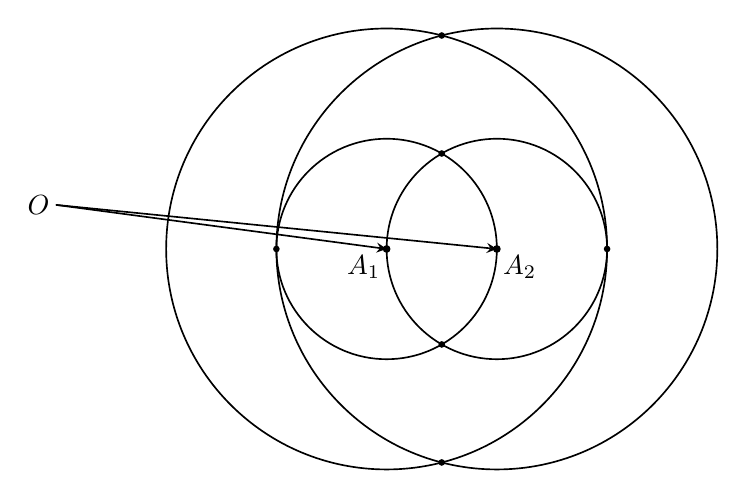
\begin{tikzpicture}[x=1.4cm,y=1.4cm,line width=.6pt,font=\normalsize]
\coordinate (O) at (-3,0.4);
\coordinate (A1) at (0,0);
\coordinate (A2) at (1,0);
\coordinate (P11a) at (0.5,0.8660254038);
\coordinate (P11b) at (0.5,-0.8660254038);
\coordinate (P22a) at (0.5,1.9364916731);
\coordinate (P22b) at (0.5,-1.9364916731);
\coordinate (P12) at (-1,0);
\coordinate (P21) at (2,0);
\draw (A1) circle[radius=1.4cm];
\draw (A1) circle[radius=2.8cm];
\draw (A2) circle[radius=1.4cm];
\draw (A2) circle[radius=2.8cm];
\draw[->,>=stealth] (O)--(A1);
\draw[->,>=stealth] (O)--(A2);
\fill (P11a) circle[radius=1.2pt];
\fill (P11b) circle[radius=1.2pt];
\fill (P22a) circle[radius=1.2pt];
\fill (P22b) circle[radius=1.2pt];
\fill (P12) circle[radius=1.2pt];
\fill (P21) circle[radius=1.2pt];
\node[left=2pt,inner sep=0pt] at (O) {$O$};
\node[below left=2pt,inner sep=0pt] at (A1) {$A_{1}$};
\node[below right=2pt,inner sep=0pt] at (A2) {$A_{2}$};

% Explicit named circle-center points, painted after all region fills.
\fill (A1) circle[radius=1.4pt];
\fill (A2) circle[radius=1.4pt];
\end{tikzpicture}
